\begin{exercise}{Précession du périhélie de Mercure}{-1}{Spé}
{meca}{centrale}

Le but de cet exercice est d'appliquer une correction post-newtonienne venant de la théorie de la relativité générale à la trajectoire de Mercure afin d'expliquer l'anomalie de la précession de la périhélie de Mercure dont une partie n'est pas expliquée par la mécanique newtonienne.

\paragraph{Résolution de problème :}~

On considère le Soleil fixé au point $O$, on notera $M$ l'emplacement de Mercure, $\vec{r} = \vec{OM}$ et $\vec{v} = \dv{\vec{r}}{t}$.

À $t = 0$, on suppose Mercure à sa périhélie, et on fixe l'origine des angles de manière à ce que $\theta = 0$ à $t=0$.

\begin{questions}
    \question En calculant la valeur du vecteur $\vec{h} = \vec{r} \cross \vec{v}$, montrer que la trajectoire de Mercure est située dans un plan contenant le Soleil et qu'elle obéit à la deuxième loi de Kepler.
    \question Quelle est la forme de la trajectoire décrite par Mercure autour du Soleil ? En utilisant les documents en annexe, donner la valeur numérique du demi-grand axe et de l'excentricité de cette trajectoire.
    \uplevel{On introduit le vecteur de Laplace $\vec{A} = \alpha \frac{\vec{r}}r + \vec{v} \cross \vec{h}$.}
    \question Montrer que pour une valeur bien choisie de $\alpha$ on a $\dv{\vec{A}}{t} = \vec{0}$. \\ On gardera cette valeur pour la suite.
    \question Calculer la norme de $\vec{A}$ en fonction de $\alpha$, $h$ et la distance Mercure-Soleil à la périhélie et montrer que le vecteur $\vec{A}$ pointe toujours vers la périhélie de Mercure.
    
    \question Montrer, en calculant $\vec{A}\cdot\vec{r}$ de deux manières différentes, l'égalité $\alpha + \frac{h^2}{r} = \norm*{\vec{A}}\cos(\theta)$.\\ En déduire $r(\theta)$. Montrer, en s'appuyant sur les documents, que la trajectoire est bien une ellipse.
    \uplevel{On souhaite retrouver la valeur de la précession (l'angle $\Delta \phi$ dont a tourné l'orbite en une révolution) de Mercure. Pour cela, on introduit une force fictive s'appliquant à Mercure en plus de l'attraction du Soleil, qui vaut $$\vec{F}_\textsc{PN}=-\gamma \frac{G m M_\odot a}{r^3}\frac{\vec{r}}{r},$$
    où $a$ est le demi-grand axe de l'orbite de Mercure, $G$ la constante gravitationnelle et $M_\odot$ la masse du Soleil.}
    \question Quelle est l'unité de $\gamma$ ? On donne $$\gamma = \frac{6 G M_\odot}{c^2a}.$$
    Estimer numériquement sa valeur. Peut on considérer $\gamma \ll 1$ ?
    \question Les résultats de la première question sont-ils toujours valables ?
    \question Calculer la nouvelle valeur de $\dv{\vec{A}}{t}$. Le vecteur $\vec{A}$ est-il toujours constant ?
    \uplevel{On définit le vecteur
    $\displaystyle \vec{u} = \frac{\vec{h} \cross \vec{A}}{hA}$
    , avec $h$ et $A$ les normes de $\vec{h}$ et $\vec{A}$, respectivement.}
    \question Quelle est la direction de $\vec{u}$ ? Sa norme ?
    \question Calculer la quantité $$\dv{\phi}{t}(\theta) = \vec{u}\vdot \dv{\vec{A}}{t}\frac{1}{A}.$$
    Que représente cette quantité ?
    \question La précession $\Delta \phi$ est donnée par la formule 
    $$\Delta \phi = \int_{(T)} \dv{\phi}{t}\dd{t} = \int_0^{2\pi}\dv{\phi}{t}\dv{t}{\theta}\dd{\theta}$$
    Interpréter cette formule et calculer la valeur de $\Delta \phi$. Est-ce cohérent avec la formule donnée en annexe ?
    \question Faire l'application numérique. La correction post-newtonienne permet-elle d'expliquer l'anomalie de la périhélie de Mercure ?
\end{questions}

\end{exercise}
\pagebreak

\printexerciseheader

\begin{center}
    \itshape --- \quad \textbf{Annexe (page 1)} \quad ---
\end{center}

\paragraph{Document 1 :}\textsf{Mercure}
\begin{center}\begin{minipage}{.9\textwidth}
Mercure est la planète la plus proche du Soleil et la moins massive du Système solaire. Son éloignement au Soleil est compris entre 0,31 et 0,47 unité astronomique (soit 46 et 70 millions de kilomètres), ce qui correspond à une excentricité orbitale de 0,2 — plus de douze fois supérieure à celle de la Terre, et de loin la plus élevée pour une planète du Système solaire. Elle est visible à l'œil nu depuis la Terre avec un diamètre apparent de 4,5 à 13 secondes d'arc. 

[...]

Comme pour l'ensemble des planètes du Système solaire, l'orbite de Mercure connaît une très lente précession du périhélie autour du Soleil, c'est-à-dire que son orbite est elle-même en rotation autour du Soleil. Cependant, contrairement aux autres planètes, la période de précession du périhélie de Mercure ne concorde pas avec les prédictions faites à l'aide de la mécanique newtonienne.

En effet, Mercure connaît une précession légèrement plus rapide que celle à laquelle on peut s'attendre en appliquant les lois de la mécanique céleste, et se trouve en avance d'environ 43 secondes d'arc par siècle. 

[...]

En 1916, Albert Einstein avance la théorie de la relativité générale. En appliquant les paramètres dits post-képlériens de sa théorie au mouvement de Mercure, Einstein fournit l'explication de la précession observée en formalisant la gravitation comme étant affectée par la courbure de l'espace-temps. La formule de précession subie par l'orbite en une période obtenue par Einstein est :

\begin{align*}
    \Delta \phi_{\text{Einstein}} = \frac{6\pi G M_\odot}{c^2 a (1-e^2)}
\end{align*}

où $a$ est le demi-grand axe de l'ellipse, $e$ son excentricité, $G$ la constante gravitationnelle, $M_\odot$ la masse du Soleil, et $c$ la vitesse de la lumière dans le vide.
\end{minipage}\end{center}
\textsl{Extrait adapté de Wikipédia, l'encyclopédie libre.}

\paragraph{Document 2 :}\textsf{La précession du périastre}
\begin{center}\begin{minipage}{.9\textwidth}
En astronomie, la précession du périastre est le phénomène selon lequel un corps en orbite autour d'un autre (par exemple une planète autour d'une étoile) voit l'ellipse décrivant sa trajectoire tourner lentement dans le plan orbital de l'objet. Cela se traduit par le fait qu'au cours des révolutions successives de l'objet, la direction décrite par la droite passant par le corps central et le corps en orbite au moment où ils sont les plus proches (le périastre) n'est pas fixe, mais varie lentement.
\end{minipage}\end{center}
\begin{figure}[H]
    \centering
    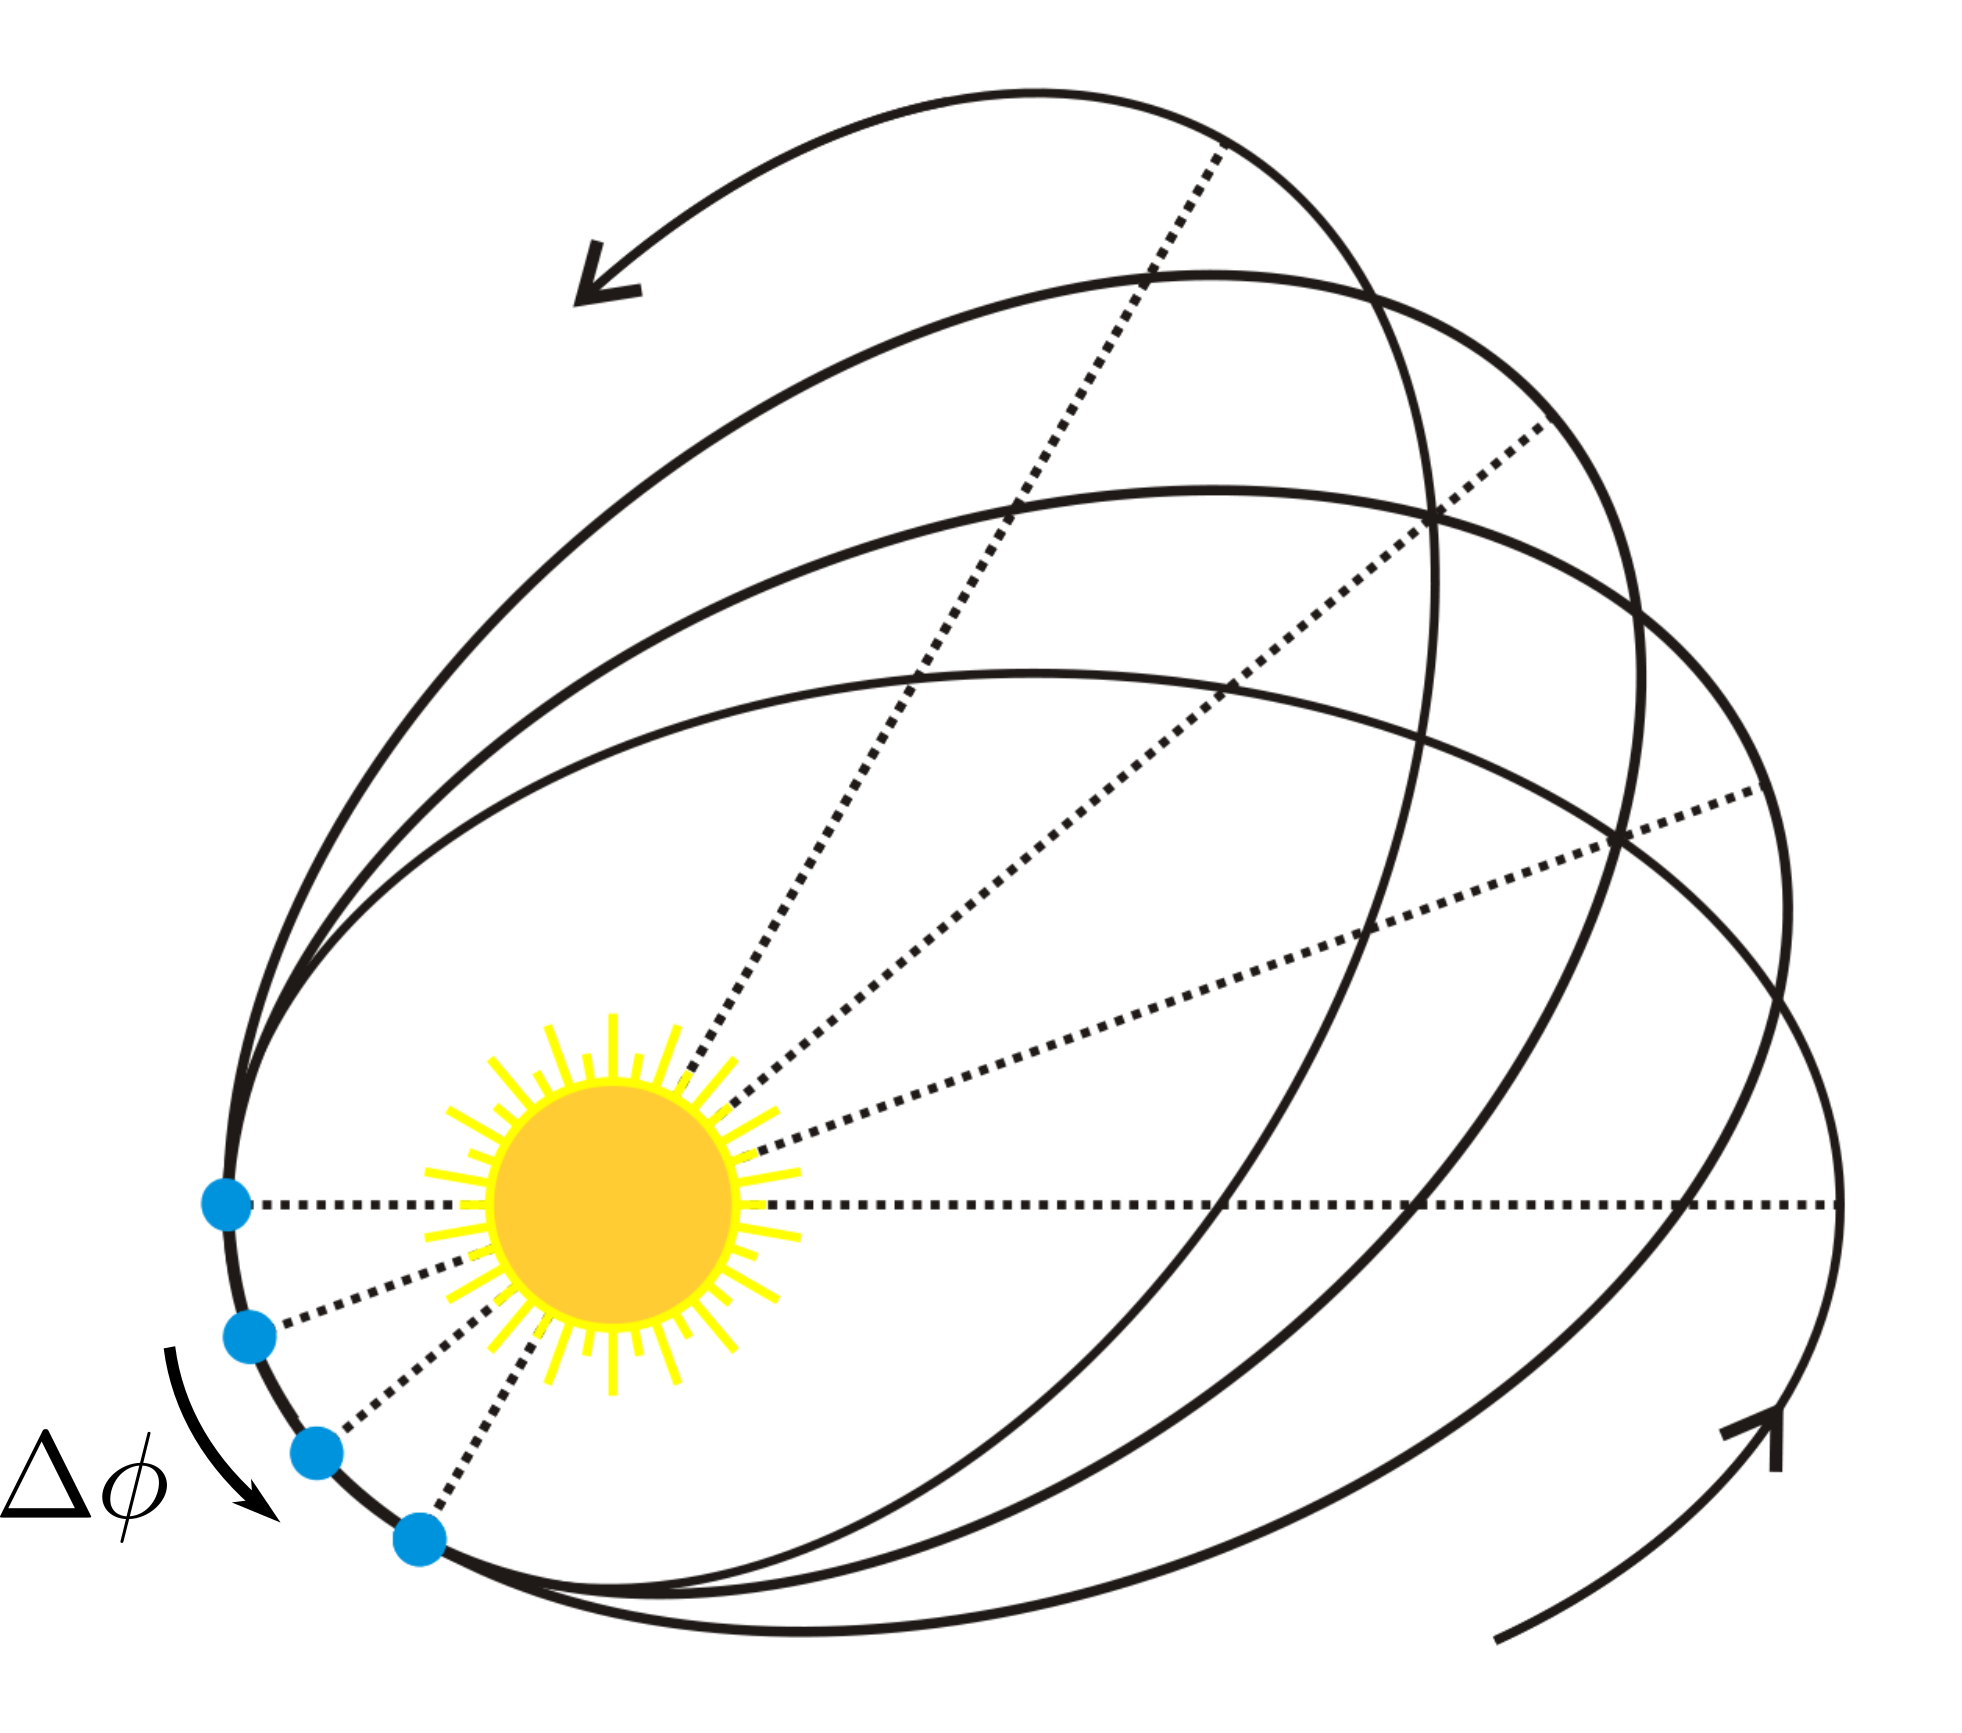
\includegraphics[width=0.3\linewidth]{oraux/centrale/perihelion_precession_dphi.png}
\end{figure}
\begin{center}\begin{minipage}{.9\textwidth}
Précession de périastre (très exagérée) : Le périastre (en bleu) tourne lentement autour de l'astre. À chaque orbite effectuée par l'objet, le périastre de déplace d'un angle $\Delta \phi$.  
\end{minipage}\end{center}
\pagebreak

\printexerciseheader

\begin{center}
    \itshape --- \quad \textbf{Annexe (page 2)} \quad ---
\end{center}

\paragraph{Document 3 :}\textsf{L'ellipse en mécanique céleste}
\begin{center}\begin{minipage}{.9\textwidth}
En mécanique képlerienne, les trajectoires des planètes sont des ellipses, dont l'un des foyers est l'astre autour duquel elles orbitent.

Pour paramétriser une ellipse dont on connaît le foyer et l'orientation du périastre, il suffit de connaître deux des grandeurs caractéristiques de l'ellipse, les autres pouvant s'en déduire facilement.

Traditionnellement, on paramétrise les ellipses en mécanique du ciel par deux grandeurs : le \textbf{demi-grand axe}, noté $a$, et l'\textbf{excentricité}, notée $e$. Le demi-grand axe est une longueur représentant l'extension spatiale de l'ellipse, tandis que l'excentricité est un nombre sans dimension compris entre 0 et 1 qui représente l'écart entre l'ellipse et un cercle (une ellipse d'excentricité 0 étant un cercle).

L'équation polaire d'une ellipse si on prend comme centre l'un des foyers est 
$$ r(\theta) = \frac{p}{1+e\cos(\theta)} $$
Où $p = a(1 - e^2)$ est appelé le \textbf{paramètre} de l'ellipse.
\end{minipage}\end{center}
\begin{figure}[H]
    \centering
    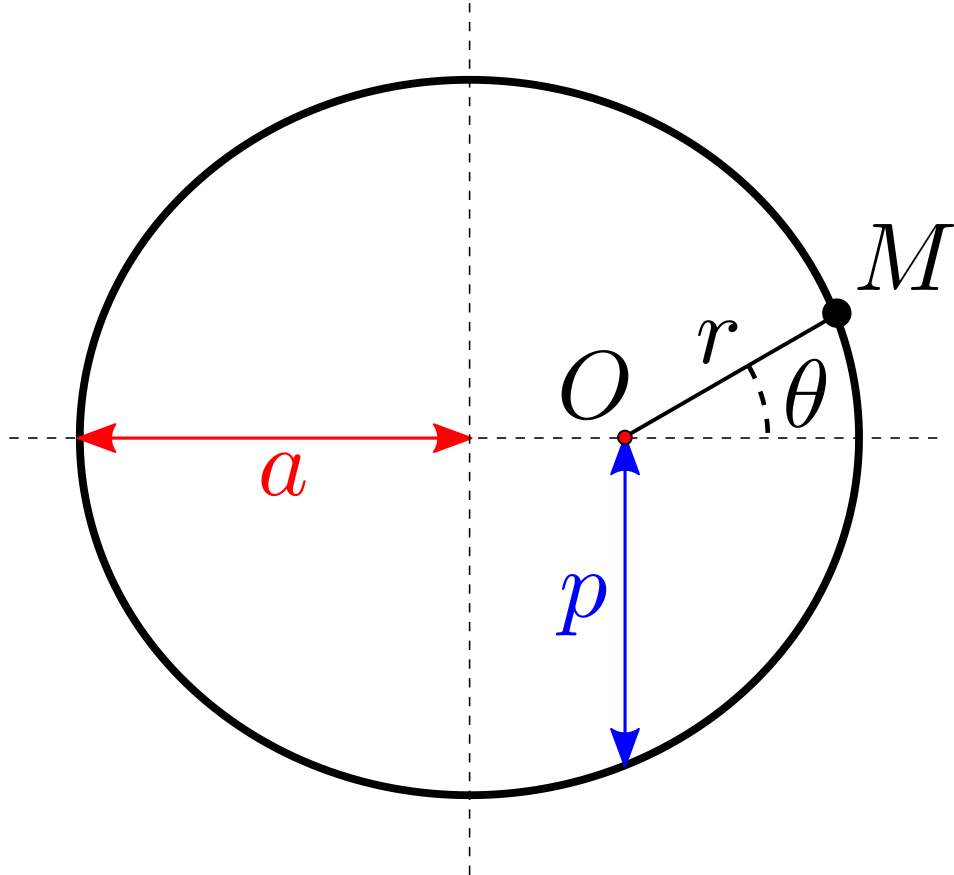
\includegraphics[width=0.4\linewidth]{oraux/centrale/EllipseVal_big.png}
\end{figure}
\begin{center}\begin{minipage}{.9\textwidth}
Paramétrisation d'une ellipse : Pour une ellipse quelconque, sont représentés le demi-grand axe $a$ et le paramètre $p$.
\end{minipage}\end{center}

\paragraph{Document 4 :}\textsf{La seconde d'arc}
\begin{center}\begin{minipage}{.9\textwidth}
La seconde d'arc correspond à une unité de mesure d'un angle. Son symbole est '', mais on peut également la noter arcsec. On l'emploie pour mesurer de très petits angles. Lorsque plus de précision est nécessaire, il est possible d'utiliser, devant l'expression seconde d'arc, les mêmes préfixes que pour les unités SI. Ainsi il existe des millisecondes d'arc, microsecondes d'arc ou encore des nanosecondes d'arc.

La seconde d'arc est définie par rapport au degré. En géométrie, on peut en effet diviser le cercle en 360 parties égales que l'on nomme degré ($ ^{\circ}$). Lorsque la mesure doit se montrer plus précise, il faut faire appel aux sous-unités du degré. La première d'entre elles est la minute d'arc ('). Comme une heure se divise en 60 minutes, un degré se divise en 60 minutes d'arc. Et comme une minute se divise en 60 secondes, une minute d'arc se divise aussi en 60 secondes d'arc. Ainsi entre le degré et la seconde d'arc, il existe un facteur 3 600, comme entre l'heure et la seconde.
\end{minipage}\end{center}
\textsl{D'après \texttt{www.futura-sciences.com}}


\paragraph{Document 5 :}\textsf{Données numériques}
\begin{itemize}
    \item Constante gravitationnelle : $6.674 \times 10^{-11}$ S.I.
    \item Masse du Soleil : $1,989 \times 10^{30}$ kg
\end{itemize}

\newpage